%% LyX 2.3.6.1 created this file.  For more info, see http://www.lyx.org/.
%% Do not edit unless you really know what you are doing.
\documentclass[twocolumn]{IEEEtran}
\usepackage[T1]{fontenc}
\usepackage[latin9]{inputenc}
\usepackage{array}
\usepackage{refstyle}
\usepackage{booktabs}
\usepackage{textcomp}
\usepackage{enumitem}
\usepackage{graphicx}
\usepackage[unicode=true,
 bookmarks=false,
 breaklinks=false,pdfborder={0 0 0},pdfborderstyle={},backref=false,colorlinks=false]
 {hyperref}
\hypersetup{pdftitle={Your Title},
 pdfauthor={Your Name},
 pdfpagelayout=OneColumn, pdfnewwindow=true, pdfstartview=XYZ, plainpages=false}

\makeatletter

%%%%%%%%%%%%%%%%%%%%%%%%%%%%%% LyX specific LaTeX commands.

\newcommand*\LyXbar{\rule[0.585ex]{1.2em}{0.25pt}}
\AtBeginDocument{\providecommand\Secref[1]{\ref{Sec:#1}}}
\AtBeginDocument{\providecommand\Figref[1]{\ref{Fig:#1}}}
\AtBeginDocument{\providecommand\Tabref[1]{\ref{Tab:#1}}}
\AtBeginDocument{\providecommand\tabref[1]{\ref{tab:#1}}}
%% Because html converters don't know tabularnewline
\providecommand{\tabularnewline}{\\}
\RS@ifundefined{subsecref}
  {\newref{subsec}{name = \RSsectxt}}
  {}
\RS@ifundefined{thmref}
  {\def\RSthmtxt{theorem~}\newref{thm}{name = \RSthmtxt}}
  {}
\RS@ifundefined{lemref}
  {\def\RSlemtxt{lemma~}\newref{lem}{name = \RSlemtxt}}
  {}


%%%%%%%%%%%%%%%%%%%%%%%%%%%%%% Textclass specific LaTeX commands.
\newlength{\lyxlabelwidth}      % auxiliary length 

%%%%%%%%%%%%%%%%%%%%%%%%%%%%%% User specified LaTeX commands.
% for subfigures/subtables
%\usepackage[caption=true,font=footnotesize]{subfig}
%\renewcommand{\thetable}{\arabic{table}}
%\renewcommand{\figurename}{Fig.}
\newref{Figure}{name = \RSFigtxt}
%\newref{tab}{name = \RSTabtxt}
%\newref{eq}{name = \RSEqtxt}
%\newcommand{\squeezeup}{\vspace{-2.5mm}}

\makeatother

\begin{document}
\title{A Time-Domain Short Circuit Study for a VSC Based Battery Energy Storage
System}
\author{Ahmad~Abdullah,~\IEEEmembership{Senior Member,~IEEE},~Muhammad~Humayun,~\IEEEmembership{Member,~IEEE},~David~Mueller,~\IEEEmembership{Member,~IEEE},
Carl~Moeller\thanks{Ahmad Abdullah (email: \protect\href{mailto:ahmad.abdullah@mortenson.com}{ahmad.abdullah@mortenson.com})
is with Faculty of Engineering at Cairo University, Cairo, Egypt and
Mortenson Construction, San Antonio, TX 78259 USA.}\thanks{Muhammad Humayun (e-mail: \protect\href{mailto:mhumayun@enernex.com}{mhumayun@enernex.com})
and David Mueller (e-mail: \protect\href{mailto:dmueller@enernex.com}{dmueller@enernex.com})
are with EnerNex, Knoxville, TN 37932 USA.}\thanks{Carl Moeller (email: \protect\href{mailto:carl.moeller@mortenson.com}{carl.moeller@mortenson.com})
are with Mortenson Construction, San Antonio, TX, 78259 USA.}\thanks{\medskip{}
\protect \\
978-1-6654-7902-8/22/\$31.00 �2022 IEEE}}
\maketitle
\begin{abstract}
A phasor domain short circuit study for a battery energy storage system
was performed per ANSI C37.010-2016. Results showed high short circuit
asymmetrical currents. Two time-domain models were also built\LyXbar{}
simplified and detailed \LyXbar to compare the results with the phasor
domain study. The results of both the simplified and the detailed
time-domain models agree to a large degree with the simplified model
on the conservative side. However, the results of both models differ
dramatically from the phasor domain model. The results in this paper
show the need to update the ANSI C37.010-2016 to account for battery
energy storage and inverter based-generation in general.
\end{abstract}

\begin{IEEEkeywords}
Electromagnetic transients, EMTDC, Energy storage, Short-circuit currents,
Storage battery, Voltage source inverters.
\end{IEEEkeywords}


\section*{NOMENCLATURE }
\noindent \begin{flushleft}
\begin{tabular}{ll}
BESS & Battery Energy Storage System\tabularnewline
MPT & Main Power Transformer\tabularnewline
MV & Medium Voltage\tabularnewline
PCS & Power Conversion Unit\tabularnewline
PMT & Padmount Transformer\tabularnewline
PWM  & Pulse-Width Modulation\tabularnewline
POI & Point of Interconnection\tabularnewline
RMS & Root Mean Square\tabularnewline
VSC & Voltage Source Converter\tabularnewline
\end{tabular}
\par\end{flushleft}

\section{Introduction\label{sec:Introduction}}

\IEEEPARstart{A}{ny} battery energy storage system (BESS) project
goes through what is known as conceptual design. This conceptual design
incorporates realistic assumptions about the grid. The most critical
assumptions are the short circuit contribution from the interconnecting
utility and the transfer power capability of the interconnecting transmission
lines. This conceptual design becomes an integral part of the financial
model of the project. This design eventually becomes complete by filling
in the details once a project developer decides to move on with the
project if a financial institution chooses to finance a project. The
conceptual design involves the determination of the ratings of the
major components of the project, such as the substation switchgear,
the main power transformer (MPT) size, and the ratings of the battery
container inverter technology, which is better known as in the industry
as power conversion unit (PCS). The PCS converts the DC battery energy
into AC energy and vice versa for charging and discharging operations. 

In this paper, we perform short circuit studies for a large BESS project
consisting of 68 voltage source converter (VSC) PCS with a total capacity
of 204 MW connected to a 230 kV substation. Each PCS contains an inverter,
switchgear, and a 0.63kV/34.5 kV 3.45 MVA padmount transformer (PMT),
all in one assembly. The studies are performed using three methods:
(1) ASPEN OneLiner phasor-domain simulation \cite{ASPEN}, (2) PSCAD�/EMTDC�
\cite{PSCAD} simplified time-domain simulations, and (3) PSCAD detailed
time-domain simulations. The comparison of the studies shows that
phasor-domain short-circuit levels are conservative as compared to
time-domain results. Also, a sensitivity analysis is carried out for
detailed time-domain simulations to show the dependencies of the short-circuit
level on the system operating and modeling conditions, e.g., BESS
connection status, MPT tap, utility source state.

The phasor domain short circuit study was done in ASPEN based on the
IEEE ANSI C37.010-1979 \cite{C37-010-1979} and IEEE Violet Book \cite{IEEEViolet}.
The IEEE ANSI C37.010-1979 is what has been historically programmed
in all phasor domain commercial short circuit packages to calculate
breaker duty ratings. The IEEE ANSI C37.010-1979 was later updated
to IEEE ANSI C37.010-2016 \cite{C37-010-2016}, and the updated version
is essentially the same. IEEE Violet Book was later updated to IEEE
3002.3-2018 \cite{IEEE3002-2-2018}. The most important aspect of
the IEEE C37.010-2016 is the multiplication factor for determining
the asymmetrical current component in case the X/R ratio is not 17.
Both IEEE standards go into depth to create sequence networks that
would produce worst case X/R ratios that tend to conservatively size
the breaker. 

Several articles have discussed fault current contributions from inverter-based
generation; however, the literature is lacking in comparing asymmetrical
fault current contributions from BESS based on the phasor and time-domain
simulation. The asymmetrical current peak of 1-5 per unit (p.u.) of
inverter\textquoteright s rated peak current for up to a quarter of
a cycle is documented in \cite{keller2010understanding,sidhu2011short,kim2019short,gonzalez2018fault}\textemdash{}
4-5 p.u. for single-phase inverters and 2-3 p.u. for three-phase inverters.
Since the asymmetrical fault characteristics of inverter-based generators
differ from conventional synchronous generators \cite{liu2018theoretical},
it is required to review and update the relevant standard for selecting
the circuit breaker capacities.A method to accurately model the symmetrical
fault contribution of the inverters is given in \cite{KIM2021106839}.
An simple iterative method to calculate inverter symmetrical short
circuit current in given in \cite{6878629}. Inverter short circuit
contribution under unbalanced fault conditions is given in \cite{liang2017short}.
The authors in \cite{9326226} study the effects of inverter based
generation on distance measurement without taking the fault decaying
DC current component into consideration. 

The paper is organized as follows: \Secref{BESS-Description} provides
details of the BESS project. The phasor domain study is given in \Secref{PhasorDomainStudy}.
The simplified and detailed time-domain studies are provided in \Secref{SimplifedEMT}
and \Secref{DetailedEMT}, respectively. \Secref{COMPARISON-OF-PHASOR}
discusses the comparison of phasor and time-domain simulations. \Secref{Conclusions}
summarizes the findings.

\section{BESS PROJECT DESCRIPTION\label{sec:BESS-Description}}

\Figref{Power-conversion-unit} shows the PCS layout used in the BESS
project under study, which is a voltage source converter PCS capable
of black-start. The PCS consists of an inverter, switchgear, and a
PMT, all in one assembly. In this sense, a PCS is more than an inverter:
it is the whole DC/AC conversion system. What makes this PCS unique
is the existence of switchgear that serves a specific function in
the overall topology. The overcurrent protection settings of this
switchgear are not adjustable due to this functionality. The switchgear
model used in this project is rated for 20 kA RMS current interruption,
while the closing and latching is 54.6 kA peak. The DC side runs at
a voltage between 900 V to 1300 V, and the AC output voltage is 630
V. The PMT is 0.63 kV/34.5 kV rated at 3.45 MVA with a vector group
of Dy1. The bushing is capable of withstanding 20 kA RMS symmetrical
current for two seconds and 52 kA peak current for ten cycles per
the IEEE C37.20.3 standard \cite{C37_20_3}. The PCS vendor rates
the whole PCS assembly for 52 kA peak withstand for ten cycles.
\begin{figure}[h]
\centering{}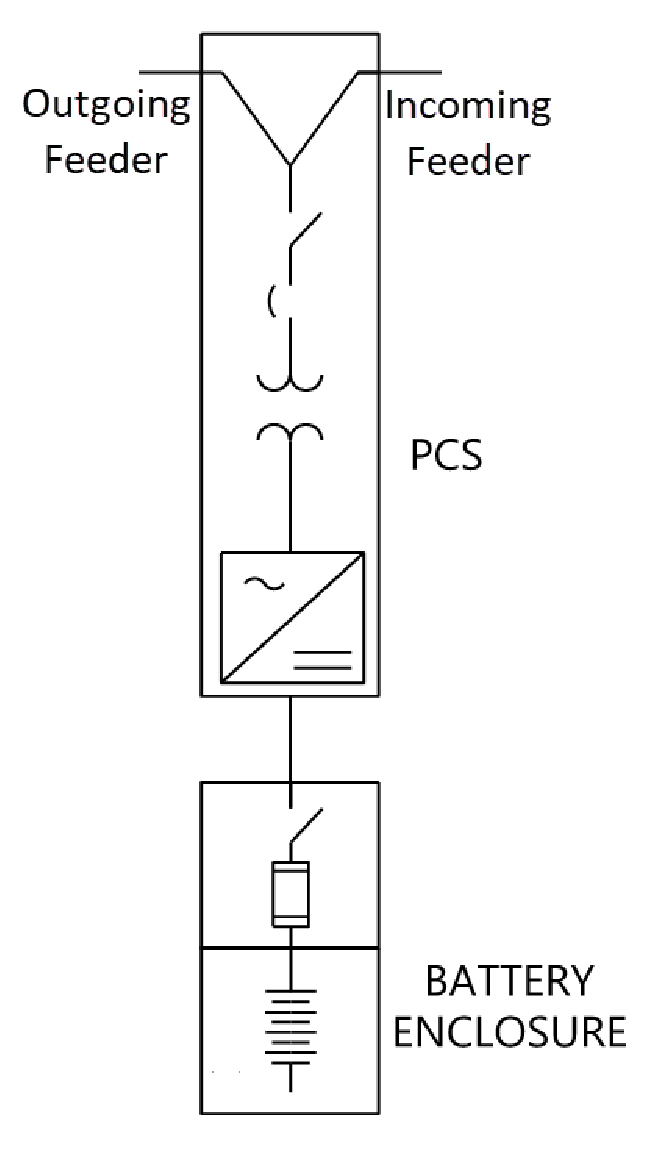
\includegraphics[scale=0.3]{Graphics/PCS}\caption{Power conversion unit (PCS) used in the battery energy storage energy
system (BESS) project under study.\label{fig:Power-conversion-unit}}
\end{figure}

The project consists of sixty-eight (68) PCSs. Each PCS is connected
to one battery enclosure. The PCSs are arranged in strings, and all
strings are connected in parallel. Each string contains several PCSs
in series, as given in \Figref{A-string-of}.
\begin{figure*}[h]
\begin{centering}
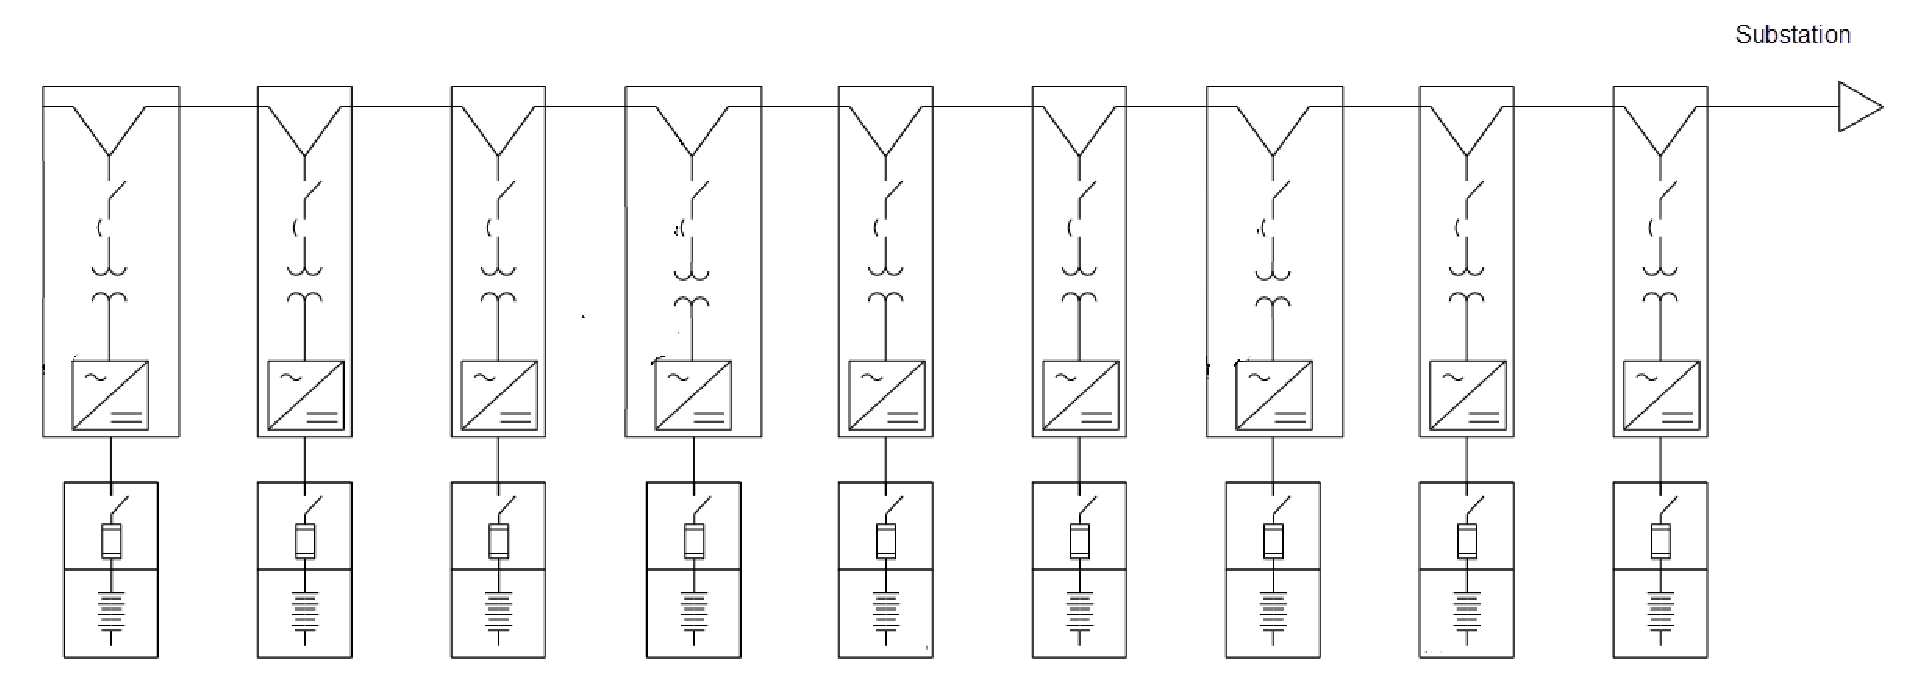
\includegraphics[scale=0.45]{Graphics/String}
\par\end{centering}
\caption{A string of PCS.\label{fig:A-string-of}}

\end{figure*}

\Figref{Interconnection-of-the} outlines the interconnection of the
BESS project under study (shown in red). The BESS project has a total
capacity of 204 MW. The MPT of this project is a three-winding transformer
that is top rated for 265 MVA. The MPT impedance is 8.4\% at the top
rating (16R tap and 16L tap impedances are 8.74\% and 8.26\%, respectively),
and the vector group is YN1yn1d1. The BESS interconnects to the transmission
grid through two 230 kV transmission lines that connect to a 500 kV
level through a 500 kV/230 kV step-up substation. The black buses
at the end of the 230 kV tie lines (floating buses on the right of
\Figref{Interconnection-of-the}) are proposed for substations for
future inverter-based generation and storage.
\begin{figure}[h]
\noindent \begin{centering}
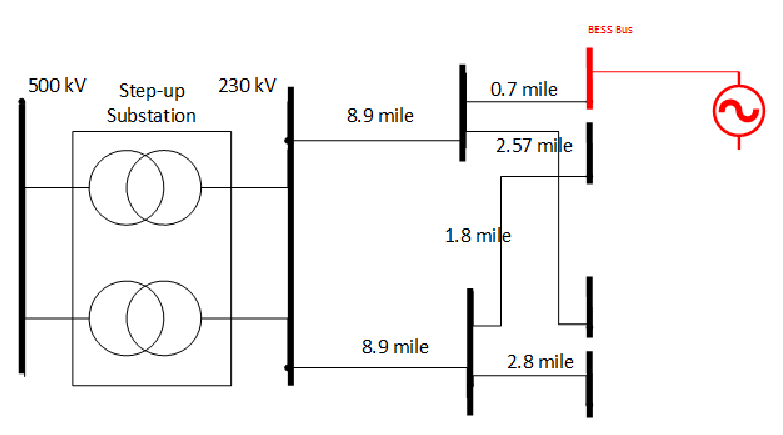
\includegraphics[scale=0.6]{Graphics/InterconnectionPic}
\par\end{centering}
\caption{Interconnection of the understudy (red) BESS project.\label{fig:Interconnection-of-the}}
\end{figure}

The original conceptual design assumed a short circuit current of
25 kA at the 230 kV bus at the step-up substation. The inverter short
circuit was considered to be 1.1 p.u. Using these assumptions, the
short circuit at the low side of the MPT within the BESS project is
24.7 kA. The designer decided to use 40 kA low side breakers. 

\Tabref{Utility-Short-Circuit} provides the utility short circuit
levels, and the PCS short circuit information is given in \Tabref{PCS-Short-Circuit}.
The first thing to notice about the current utility short circuit
is that it is very close to the assumed utility short circuit in the
conceptual design. The second thing to notice is that the inverter
steady-state short circuit contribution is one p.u., which is lower
than the assumption in the conceptual design. The third thing is that
the PCS short circuit impedance has no resistive component even though
it contains the PMT resistance. Upon contacting the PMT vendor, it
was made clear that the PCS contribution is on the 34.5 kV side and
does not include any resistance for conservative results. However,
what was not known in conceptual design stage is that the 230 kV bus
at the step-up substation can have a short circuit of 49.9 kA. The
step-up substation has two large transformers, and the grid operator
would parallel them in case of specific emergency conditions. Also,
what was not known during conceptual design is that the grid short
circuit can go up by 10 kA in case all of the projects get built in
the area.
\begin{table}[h]
\caption{Utility Short Circuit Data\label{tab:Utility-Short-Circuit}}

\centering{}%
\begin{tabular}{ccc}
\cmidrule{2-3} \cmidrule{3-3} 
 & 3-Phase Short Circuit & X/R\tabularnewline
\midrule 
Current Short Circuit & 24.5 kA & 40.94\tabularnewline
\midrule 
Maximum Build Out & 34.3 kA & 38.91\tabularnewline
\midrule 
Emergency Condition & 49.9 kA & 32.5\tabularnewline
\bottomrule
\end{tabular}
\end{table}
\begin{table}[h]
\caption{PCS Short Circuit Data\label{tab:PCS-Short-Circuit}}

\begin{centering}
\begin{tabular}{cc}
\cmidrule{2-2} 
 & Reactance\tabularnewline
\midrule 
Subtransient & 0.962 pu\tabularnewline
\midrule 
Transient & 0.99 pu\tabularnewline
\midrule 
Synchronous & 0.99 pu\tabularnewline
\bottomrule
\end{tabular}
\par\end{centering}
\end{table}


\section{PHASOR DOMAIN STUDY \label{sec:PhasorDomainStudy}}

This section describes the phasor domain modeling and short circuit
study results. 

A detailed phasor-domain short circuit study was performed using ASPEN
utilizing the grid emergency short circuit condition. The results
at the substation are given in \Tabref{Substation-Short-Circuit}.
The BESS collection system is short; thus, the fault at the first
PCS can be considered the same as the fault at the low side bus. One
thing that stands out in these results is the abnormally high X/R
ratio at the low side bus. Due to the high X/R ratios, the calculated
peak currents are also high and are given in \Tabref{Substation-Short-Circuit}
and are calculated using the equations in IEEE Std 551-2006 \cite{STD55_20106}.
The standard contains different ways of calculating the peak currents,
but it did not significantly differ. It should be noted that using
the emergency grid short circuit is not making a lot of difference
at the low side three phase short circuit because of the long tie
lines and the impedance of the MPT. 
\begin{table}[h]
\caption{Substation Short Circuit\label{tab:Substation-Short-Circuit}}

\begin{centering}
\begin{tabular}{cccc}
\cmidrule{2-4} \cmidrule{3-4} \cmidrule{4-4} 
 & 3-Phase Short Circuit & Peak Current & X/R\tabularnewline
\midrule 
230 kV High Side Bus & 20.1 kA & 53.6 kA & 16.9\tabularnewline
\midrule 
34.5 kV High Side Bus & 23.1 kA & 63.2 kA & 43.1\tabularnewline
\bottomrule
\end{tabular}
\par\end{centering}
\end{table}

Based on the results, the short circuit currents at the first PCS
on the string are higher than the PCS unit\textquoteright s rated
short circuit capability. The theoretical maximum peak current is
$2\times\sqrt{2}\times Fault~Current~RMS$. Based on that, the theoretical
maximum peak is 65.3 kA. The calculated peak current from the short
circuit study is due to the high X/R and the equations used in the
standards. Since the peak current is much higher than the capability,
a safety concern has arisen. High peak currents can cause high forces,
and the breaker may shatter. Since the peak current at the low side
in the fault study was close to the maximum theoretical, a time-domain
study was warranted to obtain more accurate results.

While the time-domain study in \Secref{SimplifedEMT} and \Secref{DetailedEMT}
were performed, the authors reached out to the PCS vendor to see if
the vendor can produce test data to verify the peak withstand of the
switchgear of the PCS. The vendor-provided data in \tabref{Vendor-Test-Data}
shows that the PCS switchgear and disconnect switch assembly can withstand
63.6 kA peak current. 

\begin{table}[h]
\caption{Vendor Test Data\label{tab:Vendor-Test-Data}}

\centering{}%
\begin{tabular}{ccccc}
\toprule 
\multicolumn{2}{c}{Phase} & R & S & T\tabularnewline
\midrule 
Applied voltage, RMS & kV & 36.18 & 36.09 & 35.05\tabularnewline
\midrule 
Making current, peak & kA & -42.48 & -63.6 & 53.41\tabularnewline
\midrule 
Making current, RMS & kA & 20.77 & 21.38 & 20.39\tabularnewline
\midrule 
Average current, 3 phases & kA & \multicolumn{3}{c}{20.85}\tabularnewline
\midrule 
Breaking current, DC comp. & \% & 1.62 & 2.40 & 1.35\tabularnewline
\midrule 
Recovery voltage, RMS & kV & 27.73 & 27.66 & 23.30\tabularnewline
\midrule 
TRV, peak & kV & -51.9 & -46.8 & -37.2\tabularnewline
\midrule 
Arc duration & s & 0.005 & 0.011 & 0.011\tabularnewline
\midrule 
Opening time & s & \multicolumn{3}{c}{0.081}\tabularnewline
\midrule 
Breaking time & s & 0.086 & 0.092 & 0.092\tabularnewline
\bottomrule
\end{tabular}
\end{table}


\section{SIMPLIFIED TIME-DOMAIN MODEL\label{sec:SimplifedEMT}}

This section describes the simplified time-domain modeling and short
circuit study results. PSCAD, a general-purpose time-domain simulation
tool for studying the transient behavior of electrical networks, is
used for the simulations. 

For this study, the phasor-domain short circuit study model of \Secref{PhasorDomainStudy}
was converted to a time-domain model. All transmission lines and underground
cables were converted to pi-equivalent segments. The grid was represented
as an ideal voltage source behind an impedance. The impedance was
chosen to produce the emergency condition fault current at the 230
kV point of interconnection (POI) bus. The PCS was represented as
an ideal voltage behind a 0.962 pu impedance at the 34.5 kV level.
The purpose of the time-domain study is to:
\begin{enumerate}
\item Quantify the effect of the cable and transmission line charging capacitance
\item Obtain a more realistic estimate of the peak current
\item Perform a sensitivity study regarding the MPT tap changer, transmission
line temperature, and generation level in the project 
\end{enumerate}
A worst-case analysis showed that the peak current is 57 kA and is
shown in \Figref{Simplified-PSCAD-Study}. This is 10\% less than
the phasor domain short circuit study. For this reason, it was decided
to perform a detailed time-domain analysis that considers the PCS
inverter response and this is given in the next section.
\begin{figure}[h]
\centering{}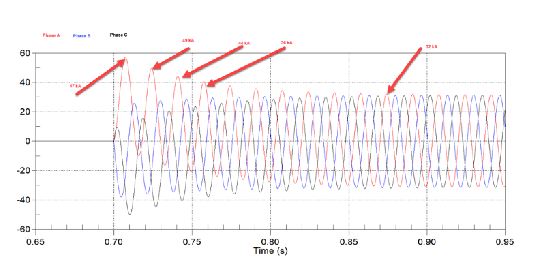
\includegraphics{Graphics/simplifiedPscadstudy}\caption{Fault current using simplified PSCAD study.\label{fig:Simplified-PSCAD-Study}}
\end{figure}


\section{DETAILED TIME-DOMAIN MODEL \label{sec:DetailedEMT}}

This section describes the detailed PSCAD time-domain modeling, simulated
cases, and short circuit study results. 

\subsection{PCS Model Benchmarking\label{subsec:PCS-Model-Benchmarking}}

The PCS vendor provided the PSCAD model, which can be parameterized
to represent a single PCS and an aggregated model of the whole BESS.
It should be noted that the vendor PSCAD model contains a transformer
with zero resistance as well. First, the single PCS model short-circuit
contributions are validated with the laboratory-tested values by applying
a three-phase-to-ground fault on the medium voltage (MV) side. \Figref{Single-PCS-current},
\Figref{Currents_Low-voltage-side-of_PCS}, and \Figref{Currents-at-theLVofPMT}
show the simulated results\LyXbar (1) currents at the MV side, (2)
currents at the low-voltage side, (3) pulse-width modulation (PWM)
output voltage, and (4) power frequency filtered PWM output voltage.
The figures display that a current spike of 1.87 p.u. appears for
a short duration because inverter control takes around 200 \textmu s
to decrease PWM average voltage \cite{turcotte2009fault,PWM}. This
decrease in average voltage is by inverter controls to protect it
from damage due to overcurrent. These simulated results match well
with the PCS laboratory tests as given in \Figref{Single-PCS-laboratory}.
\begin{figure}[h]
\begin{centering}
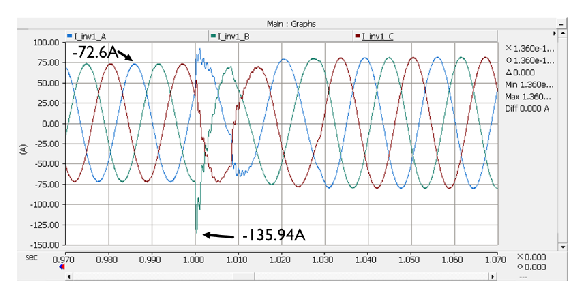
\includegraphics[scale=0.95]{Graphics/fig5}\caption{Single PCS current contribution of detailed PSCAD model (all phases)
at the MV side for a 3-phase-to-ground fault on the MV side at 1 second.\label{fig:Single-PCS-current}}
\par\end{centering}
\end{figure}
\begin{figure}[h]
\begin{centering}
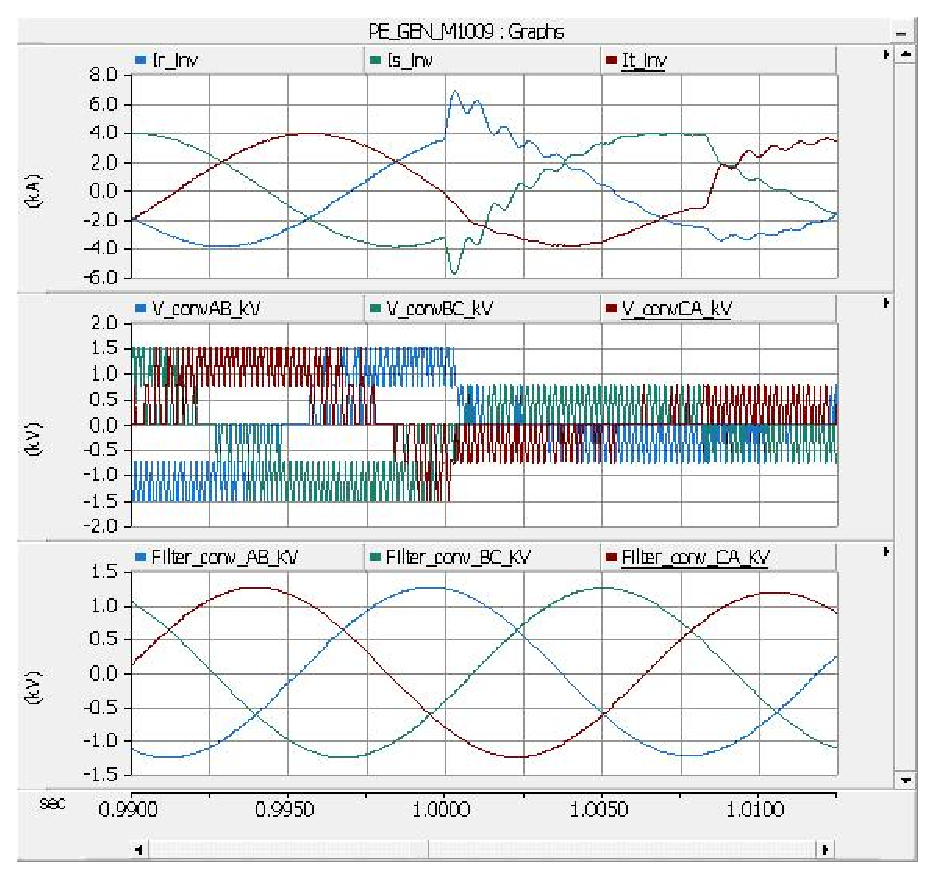
\includegraphics[scale=0.58]{Graphics/fig6}\caption{Currents using detailed PSCAD model at the low-voltage side (top),
PWM output voltage (middle), PWM output voltage filtered for power
frequency (bottom).\label{fig:Currents_Low-voltage-side-of_PCS}}
\par\end{centering}
\end{figure}
\begin{figure}[h]
\begin{centering}
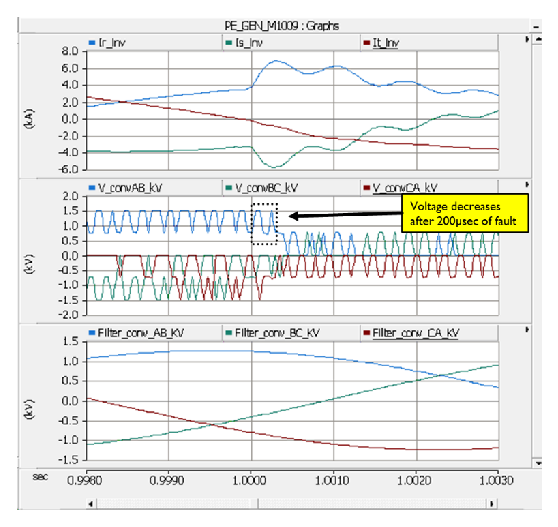
\includegraphics[scale=0.97]{Graphics/fig7}\caption{Currents using detailed PSCAD model at the low-voltage side of the
PMT (top), PWM output voltage (middle), PWM output voltage filtered
for power frequency (bottom).\label{fig:Currents-at-theLVofPMT}}
\par\end{centering}
\end{figure}
\begin{figure}[h]
\begin{centering}
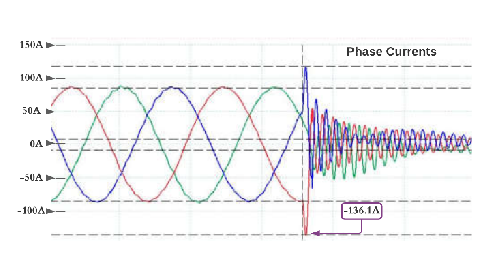
\includegraphics[scale=1.15]{Graphics/fig8}
\par\end{centering}
\caption{Single PCS laboratory test current measurements at the MV side of
the PMT for a 3-phase-to-ground fault on the MV side.\label{fig:Single-PCS-laboratory}}
\end{figure}


\subsection{PCS Reduced Order Model\label{subsec:PCS-Reduced-Order}}

The vendor-provided PCS model has a limitation that only six to seven
instances can be executed using a typical computer. Therefore, the
PCS aggregation approach is adopted to perform simulation for the
BESS project\LyXbar a single equivalent PCS model is used for multiple
instances by changing the parameters following the vendor instructions.

The short circuit contributions of four and eight PCS instances and
their equivalent aggregates are validated by applying a three-phase-to-ground
fault at 1 s on the MV side of the PMT. A one second is used to ensure
that the models have reached steady state before introducing the fault.
In the multiple instances case, a short (50 ft) 500 kcmil cable is
also considered between inverters to imitate the actual field installation.
\Figref{Simulation-setup-for}, \Figref{SimulationOf9PCS}, \Figref{Fault-contributions-from4pcs}
and \Figref{Fault-contributions-from8PCS} show the simulation setups
and results. The total fault contributions are approximately the same
as their model equivalents for both four and eight PCS instances.
\begin{figure}[h]
\begin{centering}
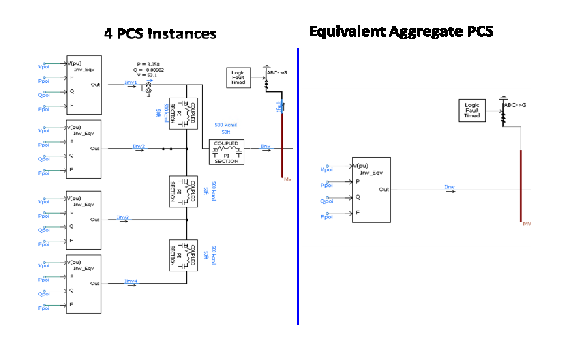
\includegraphics{Graphics/fig9}
\par\end{centering}
\caption{Simulation setup for 4 PCS instances vs. aggregate model.\label{fig:Simulation-setup-for}}

\end{figure}
\begin{figure}[h]
\begin{centering}
\includegraphics[scale=0.38]{Graphics/8PCS}\caption{Simulation setup for 8 PCS instances vs. aggregate model.\label{fig:SimulationOf9PCS}}
\par\end{centering}
\end{figure}
\begin{figure}[h]
\begin{centering}
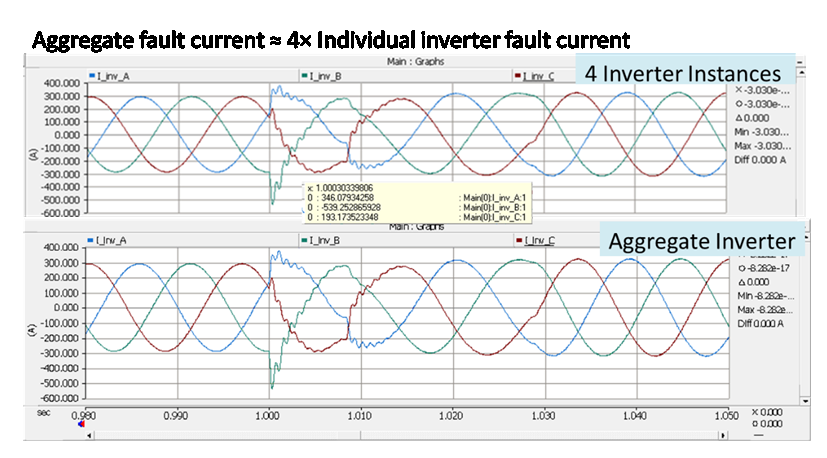
\includegraphics[scale=0.67]{Graphics/fig10}\caption{Fault contributions from 4 PCS instances vs. aggregate model.\label{fig:Fault-contributions-from4pcs}}
\par\end{centering}
\end{figure}
\begin{figure}[h]
\begin{centering}
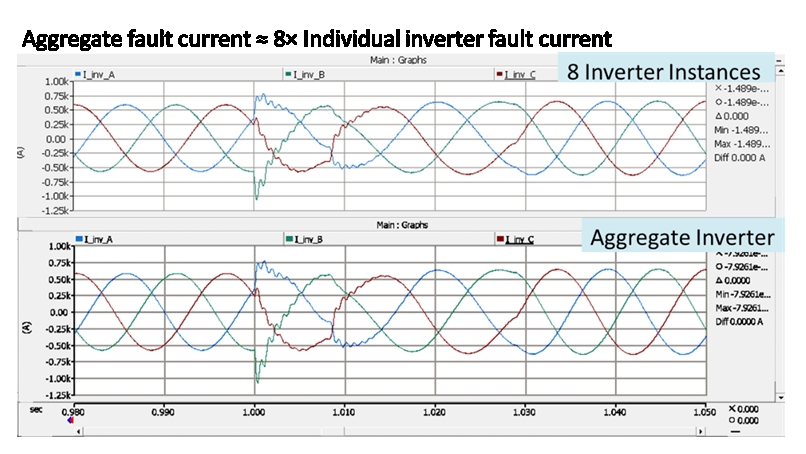
\includegraphics[scale=0.68]{Graphics/fig12}\caption{Fault contributions from 8 PCS instances vs. aggregate model.\label{fig:Fault-contributions-from8PCS}}
\par\end{centering}
\end{figure}


\subsection{System Model\label{subsec:System-Model}}

\Figref{Snapshot-of-the} shows the PSCAD snapshot of the system model
setup. A 230 kV voltage source equivalent is used for the system upstream
of POI. The system model consists of two 230 kV transmission line
sections, MPT, and two 34.5 kV short MV cable sections, and 68 PCS\textquoteright{}
equivalent aggregate 233.24 MVA BESS. The accuracy of the PSCAD simulation
model was verified using steady-state quantities, such as bus voltages
and the collection cable charging MVAR. 
\begin{figure*}[h]
\begin{centering}
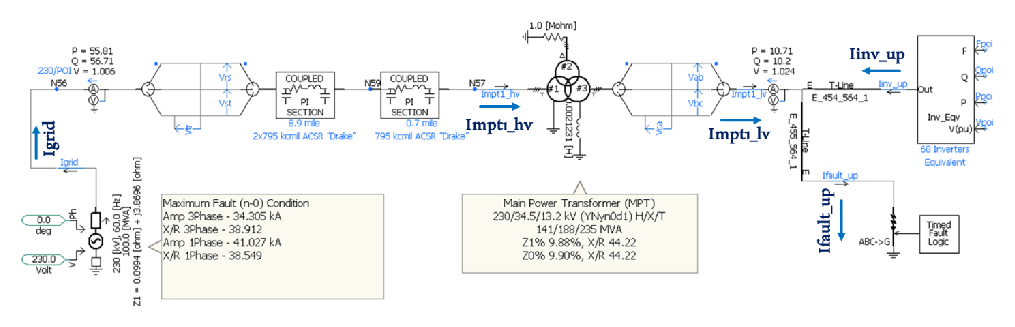
\includegraphics{Graphics/fig13}\caption{Snapshot of the detailed PSCAD model setup for the study.\label{fig:Snapshot-of-the}}
\par\end{centering}
\end{figure*}


\subsection{Study Cases\label{subsec:Study-Cases}}

\Tabref{Case-list-for} shows six case studies that are performed
for a three-phase-to-ground fault on the 34.5 kV BESS collector system.
Case 1 is the base case that considers all PCS of BESS, transmission
capacitance, ultimate build-out utility bus 34.3 kA fault level, and
neutral tap for MPT. The other cases are for sensitivity analysis
to find the dependencies of the short-circuit current on the system
operating and modeling conditions. The sequence of events for the
simulation are:
\begin{itemize}
\item t = 0-1 s: Simulation starts and steady-state operation
\item t = 1 s: Three-phase-to-ground fault on 34.5 kV BESS collector system 
\end{itemize}
For this study, the inverter voltage and frequency protection and
power plant controller functions (e.g., voltage, reactive power, frequency,
power factor control modes) are disabled to ensure worst case results
are obtained. 
\begin{table}[h]
\caption{Case list for detailed time-domain simulations\label{tab:Case-list-for}}

\centering{}%
\begin{tabular}{cc>{\centering}p{1.5cm}>{\centering}p{1cm}>{\centering}p{1cm}}
\toprule 
Case & Number of PCS & Transmission Capacitance & Utility Fault kA & MPT Tap\tabularnewline
\midrule 
1 & 68 & Yes & 34.3 & N\tabularnewline
\midrule 
2 & 0 & Yes & 34.3 & N\tabularnewline
\midrule 
3 & 0 & No & 34.3 & N\tabularnewline
\midrule 
4 & 68 & Yes & 49.9 & N\tabularnewline
\midrule 
5 & 68 & Yes & 34.3 & 16R\tabularnewline
\midrule 
6 & 68 & Yes & 34.3 & 16L\tabularnewline
\bottomrule
\end{tabular}
\end{table}


\subsection{Results\label{subsec:Results}}

This section furnishes short circuit contribution results for all
cases in \Tabref{Case-list-for}. 

\subsubsection{Case 1\label{subsec:Case-1}}

\Figref{Case-1-fault} shows the total fault current, contributions
from the 68 inverters, and contribution from the grid for a three-phase-to-ground
fault at BESS collector systems. The following observations can be
made from the figure:
\begin{itemize}
\item Inverters slightly increase the asymmetrical fault current peak (first
peak after the fault at 1 s)\LyXbar total 51.5 kA, utility contribution
50.6 kA, and inverter contribution 9.1 kA. It should be noted the
peak inverter contribution is negative while the grid is positive. 
\item The contributions of the inverters in symmetrical fault current peak
(after a few cycles from the fault) are higher\LyXbar{} total 33.1
kA, utility contribution 27.7 kA, and inverter contribution 5.5 kA.
The inverter contributions are equal to around one p.u. of their ratings.
\begin{figure}[h]
\begin{centering}
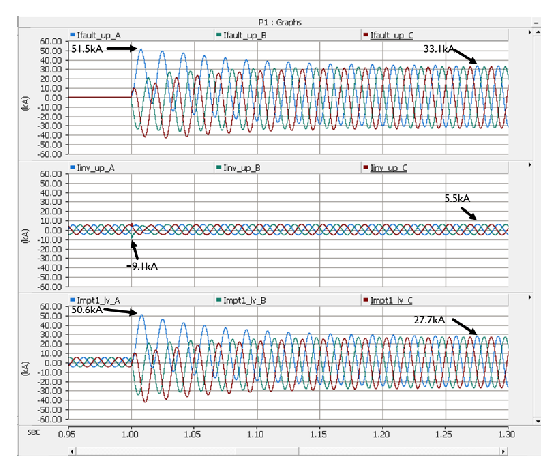
\includegraphics[scale=0.98]{Graphics/fig14}\caption{Case 1 fault currents: Total current (top), inverter contributions
(middle), and utility grid contribution (bottom).\label{fig:Case-1-fault}}
\par\end{centering}
\end{figure}
\end{itemize}

\subsubsection{Sensitivity Analysis Results\label{subsec:Sensitivity-Analysis-Results}}

\Tabref{Asymmetric-peak-fault} displays the asymmetrical peak fault
current for all the cases. The results indicate that:
\begin{itemize}
\item Case 1-Case 3: The presence of inverters in the system and not modeling
transmission line capacitance decrease the asymmetrical peak fault
current slightly (by 0.1 kA; from 51.5 kA to 51.4 kA). This means
that ignoring system capacitance per ANSI short circuit procedures
is not making tangible difference. 
\item Case 4: Intuitively, a higher source fault level results in higher
fault currents. Even though there is 15 kA difference in grid contribution,
this is only causing a 1.5 kA difference at the low side of the MPT. 
\item Case 5 and Case 6: Changing the tap of the MPT decreases (by 0.7 kA
for 16R and 1.9 kA for 16L) the asymmetrical peak fault current compared
to Case 1 due to relatively higher impedance for 16R tap and lower
source voltage for 16L tap. The function of the taps is to bring the
source side voltage to the desired (e.g., one p.u.) voltage at the
low side of the MPT. Both tap selection and source voltage settings
influence the fault current. The impedance of the MPT directly (nonlinear)
depends on the number of windings that change with the tap position\textemdash{}
impedance is the highest for tap 16R and the lowest for 16L. In the
simulation, the 16R tap steps down the relatively higher source voltage
(compared to Case 1) to the one p.u. Consequently, the decrease in
fault current due to higher impedance dominates the increase in current
because of the higher source voltage. Contrarily, for the 16L tap,
the decrease in fault current due to relatively lower source voltage
(compared to Case 1) is dominating the increase in current because
of lower winding impedance. This converse behavior domination of impedance
and source voltage on fault current for different taps is because
of nonlinear MPT impedance relation with the changes in the number
of windings. 
\begin{table}[h]
\caption{Asymmetric peak fault current\label{tab:Asymmetric-peak-fault}}

\begin{centering}
\begin{tabular}{c>{\centering}m{5cm}>{\centering}p{2cm}}
\toprule 
Case & Case Description & Asymmetrical Peak kA\tabularnewline
\midrule 
1 & 68 PCS; Tie line capacitance; Utility fault level: 34.305 kA; MPT
Tap: N & 51.5\tabularnewline
\midrule 
2 & No PCS & 51.4\tabularnewline
\midrule 
3 & No PCS; No transmission line capacitance & 51.4\tabularnewline
\midrule 
4 & Emergency higher fault level (49.9) at the source & 53\tabularnewline
\midrule 
5 & MPT tap at 16R & 50.8\tabularnewline
\midrule 
6 & MPT tap at 16L & 49.6\tabularnewline
\bottomrule
\end{tabular}
\par\end{centering}
\end{table}
\end{itemize}

\section{COMPARISON OF PHASOR AND TIME-DOMAIN RESULTS\label{sec:COMPARISON-OF-PHASOR}}

Table VII presents the comparison between asymmetrical peak fault
current for a three-phase-to-ground fault on 34.5 kV BESS collector
system with emergency fault level condition at the utility source
side. The phasor-domain analysis depicts the highest (63.2 kA) fault
current, followed by the simplified (57 kA) and detailed (53 kA) time-domain
analyses values. 
\begin{table}[h]
\caption{Asymmetric peak fault current for emergency fault level\label{tab:Asymmetric-peak-fault-1}}

\centering{}%
\begin{tabular}{cc}
\toprule 
Model & Asymmetrical Peak kA\tabularnewline
\midrule 
Phasor-domain & 63.2\tabularnewline
\midrule 
Simplified time-domain & 57\tabularnewline
\midrule 
Detailed time-domain & 53\tabularnewline
\bottomrule
\end{tabular}
\end{table}

The difference in asymmetrical current is solely due to the inverter
contribution which is not mentioned in the standards. It is the authors'
experience that the inverters do not contribute any substantial asymmetrical
current regardless of their technology. This stems from the fact that
the PWM control reacts fast to control the current to protect the
inverter components. In this paper, it is clear from the simulations
that the high X/R ratio is causing a conservative asymmetrical current.
The C37.010-2016 calls for a 20\% margin in switchgear sizing. The
results of this paper shows that IEEE calculations adds another 10\%
margin. This 30\% margin is making it more expensive to design renewable
energy projects. 

In the end, a costly decision was made to redesign the project substation
to include current limiting reactors to limit the grid short circuit
contribution to limit the asymmetrical current. The main reason for
that decision was that the study performed in this paper was out of
step with the IEEE standards and the project's owner did not want
to take risks even if it were based on deep engineering analysis.
This shows the need to update the related IEEE standards to include
inverter short circuit behavior. 

\section{Conclusions \label{sec:Conclusions}}

This paper has compared the fault current for a large 204 MW BESS
project calculated using three methods: (1) ASPEN phasor-domain simulation,
(2) PSCAD simplified time-domain simulations, and (3) PSCAD detailed
time-domain simulations. The comparison indicated that phasor-domain
short-circuit asymmetrical peak levels are conservative as compared
to time-domain results. 

Furthermore, sensitivity analysis results have shown that PCSs do
not increase the asymmetrical peak current significantly. Moreover,
the results exhibited that the inverter contributions to symmetrical
fault current are equal to around one p.u. of their ratings. Also,
for the project under study, the operating conditions of the MPT tap
position decreased the asymmetric peak, and modeling of transmission
line capacitance did not change the peak current significantly. 

The results of this paper shows the need to update the IEEE standards
to include the right way of modeling inverter short circuit contribution. 

\bibliographystyle{IEEEtran}
\bibliography{References}

\end{document}
